\documentclass[10pt,twocolumn,letterpaper]{article}

\usepackage{cvpr}
\usepackage{times}
\usepackage{epsfig}
\usepackage{graphicx}
\usepackage{amsmath}
\usepackage{amssymb}

% Include other packages here, before hyperref.

% If you comment hyperref and then uncomment it, you should delete
% egpaper.aux before re-running latex.  (Or just hit 'q' on the first latex
% run, let it finish, and you should be clear).
\usepackage[breaklinks=true,bookmarks=false]{hyperref}

\cvprfinalcopy % *** Uncomment this line for the final submission

\def\cvprPaperID{****} % *** Enter the CVPR Paper ID here
\def\httilde{\mbox{\tt\raisebox{-.5ex}{\symbol{126}}}}

% Pages are numbered in submission mode, and unnumbered in camera-ready
%\ifcvprfinal\pagestyle{empty}\fi
\setcounter{page}{1}
\begin{document}

%%%%%%%%% TITLE
\title{3D Object Classification Using Deep Learning}

\author{Abhilash Sunder Raj\\
Stanford University\\
{\tt\small abhisr@stanford.edu}
% For a paper whose authors are all at the same institution,
% omit the following lines up until the closing ``}''.
% Additional authors and addresses can be added with ``\and'',
% just like the second author.
% To save space, use either the email address or home page, not both
\and
Ameya Joshi\\
Stanford University\\
{\tt\small josame@stanford.edu}
\and
Vishakh Hegde\\
Stanford University\\
{\tt\small vishakh@stanford.edu}
}


\maketitle
%\thispagestyle{empty}

%%%%%%%%% ABSTRACT
\begin{abstract}
This project aims to study, explore and implement 2D convolutional neural networks (CNNs) to classify 3D objects. We give a short introduction, convey the motivation, describe related work and talk about the methods we employed to solve this problem. Thereafter, we introduce the data set and analyze the performance of several models we train. Finally, we implement transfer learning by way of a SVM trained on the hidden features rendered by our network. 
\end{abstract}

%%%%%%%%% BODY TEXT
\section{Introduction}

In the digital age, there is a treasure trove of information available all around us in the form of images and videos. However, most of this visual information is captured in only two dimensions. The real world has three dimensions, and very little data is available that captures the third dimension - depth. There is a critical requirement for most Augmented Reality systems to have a depth sensor as well, to understand the real world better, before making an attempt to augment it. Even for Virtual Reality content creation, there is a need to have cameras that capture 3D information of the scene. Realizing this, companies like Microsoft and Intel have been developing affordable consumer devices like Kinect and RealSense that have a depth sensor along with a standard RGB image sensor. Thanks to their efforts, there are many such consumer cameras available today, at affordable prices.
\\
These cameras allow us to generate 3D models of real world objects. Judging by the current interest in this field, it is a safe bet that the world will soon move from conventional 2D imaging to 3D imaging. Companies which build depth cameras and software to create 3D object models will need technology to analyze and make sense of their depth images. Recognizing this, we decided to explore the possibility of creating an application which can classify 3D object models. Such an application will have many use-cases. We can automatically detect and classify objects seen by 3D cameras of an Augmented Reality system. Another key application area is e-commerce. A growing number of e-commerce companies and start-ups are working on capturing, processing, storing and displaying depth images on e-commerce websites, in order to improve the user experience.
\\
In this project, we try to explore and implement classification on three-dimensional objects using CNNs. State of the art algorithms for 3D object classification are different from those used for 2D object classification. Therefore, we cannot use existing and off-the-shelf 2D image classification technologies for 3D objects. One of the primary reasons for this is that 3D objects have different representations (unlike 2D images, where RGB format is a standard). In order to deal with this issue, we have constructed and implemented our own CNN.
\\
The input to our system is a 3D CAD model of the query object. This is first converted to a $30\times30\times30$ binary voxel. This voxel is the input to our CNN. We then use a CNN with 2D convolutions to output one out of 40 possible class labels to which we think the query object most likely belongs. We also train a SVM on the hidden layer features and output one out of 40 possible class labels. These input features are obtained from the CNN that we train in the previous step.
%-------------------------------------------------------------------------
\section{Related Work}
Classification of 3D objects has been proposed using hand-crafted features along with a machine learning classifier in ~\cite{lai20093d}, ~\cite{teichman2011towards} and ~\cite{behley2012performance}. With the advent of deep learning, a lot of research has revolved around classifying RGB-D images using CNNs. ~\cite{hoft2014fast},~\cite{socher2012convolutional}, ~\cite{lenz2015deep} and ~\cite{gupta2014learning} propose novel 3D object recognition techniques by using CNNs and RNNs on RGB-D images. 
However, more recently, the focus of research has also included finding better ways to represent 3D data. In a way, better representation has enabled better classification.
The creators of the ModelNet40 dataset have proposed a representation and a 3D CNN to classify 3D objects in ~\cite{Authors14}. In ~\cite{voxnet}, the authors have proposed a 3D CNN and have tested their algorithm on LIDAR and CAD data. ~\cite{deeppano} suggests a new robust representation of 3D data by way of a cylindrical panoramic projection that is learned using CNNs. The authors tested their panoramic representation on the ModelNet40 dataset and outperformed typical methods when they published their work. However, the state-of-the-art technique for 3D object classification has been proposed in ~\cite{Authors14b}. The authors propose a novel representation of 3D data which includes generating 2D projections of the 3D object from different views. CNNs are then trained on the 2D data. This method has attained 90.1\% classification accuracy on the ModelNet40 dataset. The problem with hand-designed 3D shape descriptors is that they tend to be very high-dimensional, making classifiers prone to overfitting due to the so-called 'curse of dimensionality'. On the other hand, view-based descriptors proposed in ~\cite{Authors14b} have a number of desirable properties: they are relatively low-dimensional, efficient to evaluate, and robust to 3D shape representation artifacts, such as holes, imperfect polygon mesh tessellations, noisy surfaces. The rendered shape views can also be directly compared with other 2D images, silhouettes or even hand-drawn sketches. The RGB-D approach does not make full use of the geometric information in the data and makes it difficult to integrate information across viewpoints. The strength of using 3D voxel data for classification as proposed in ~\cite{Authors14} is that such models not only can predict classes but can jointly hallucinate missing structures and also allow us to build an active recognition system to choose an optimal subsequent view for observation, when the category recognition from the first view is not sufficiently confident.
%-------------------------------------------------------------------------
\section{Methods}
\label{sec:methods_section}
The general approach to solving the 3D object classification problem involves two steps namely, coming up with a representation for the 3D data and training a CNN/RNN on that representation of the data. We decided to go ahead with the voxel representation proposed in ~\cite{Authors14}, so that we could spend more time on learning how to train and test CNNs instead of focusing on what a good representation for 3D data would be. Once we had fixed the representation, we again had two choices, using 2D convolutions or using 3D convolutions. We realized that having an efficient way of training CNNs (in terms of execution time and memory usage) is critical for the success of this project, as a lot of different models need to be trained and different combinations of hyper-parameters need to be tested. There are already many libraries that can efficiently perform 2D convolutions, for example - Caffe ~\cite{jia2014caffe} and we decided to go ahead with its efficient GPU implementations instead of writing efficient code for performing 3D convolutions. Hence we decided to use 2D convolutions for classifying 3D objects. All of our models were trained on Amazon AWS GPU instances.
\subsection{Model selection}
Since ModelNet40 ~\cite{Authors14} is a relatively new dataset, there aren't too many publicly known pre-trained models for 2D convolution on the 3D voxel data. Also, almost every approach to solve the classification problem on this data involves a unique representation of the 3D data, for example ~\cite{deeppano}. This prompted us to try different architectures, learn how the validation accuracy responds to changes in the architecture and finally propose a good architecture for this representation of the problem. As part of this project, we have trained 20 different models having 11 different architectures. 
\subsubsection{Baseline architecture}
We used the three-layer-net written as part of the CS 231n assignments as our baseline model. The architecture is : ReLU - $2 \times 2$ max pool - affine - ReLU - affine - softmax. The softmax loss for the $i^{th}$ training example is given by:
\begin{equation}
L_i = -f_{y_{i}} + \log \sum\limits_{j} e^{f_j} 
\end{equation}
where ${f_j}$ means the $j^{th}$ element of the vector of class scores $f$. The full loss for the dataset is the mean of $L_i$
 over all training examples together with a regularization term $R(W)$. The Adam update rule ~\cite{kingma2014adam} is given by:
\begin{equation}
m=\beta_1*m + (1-\beta_1) * dx
\end{equation}

\begin{equation}
v=\beta_2*v + (1-\beta_2) * dx^2
\end{equation}

\begin{equation}
x+= \frac{- learning\_rate * m}{eps + \sqrt[2]{v}}
\end{equation}

\subsubsection{Novel architectures}
All of the novel models were trained in Caffe ~\cite{jia2014caffe} using the softmax loss and the Stochastic Gradient Descent (SGD) with momentum solver, with a momentum of 0.9. SGD with momentum is given by: 
\begin{equation}
\nu = \gamma*\nu + \alpha*\Delta_{\theta}J(\theta; x^{i}, y^{i})
\end{equation}

\begin{equation}
\theta = \theta - \nu
\end{equation}
\\where:
\\$J(\theta)$ is the objective function\\
$(x^{i}, y^{i})$ is the training example\\
$\nu$ is the velocity vector\\
$\alpha$ is the learning rate\\
$\gamma$ determines for how many iterations the previous gradients are incorporated into the current update\\
\\If the objective has the form of a long shallow ravine leading to the optimum and steep walls on the sides, standard SGD will tend to oscillate across the narrow ravine since the negative gradient will point down one of the steep sides rather than along the ravine towards the optimum. The objectives of deep architectures have this form near local optima and thus standard SGD can lead to very slow convergence particularly after the initial steep gains. Momentum is one method for pushing the objective more quickly along the shallow ravine and hence we have used it in our models ~\cite{sgdmom}.
We used the 'step' learning rate policy and weight decay for regularization. Our batch size for training is 256 and for testing is 250. We observed that increasing the batch size increased the GPU memory usage. Also, most of the popular models like AlexNet and BVLC reference caffenet used a batch size of 256. To start off we chose a batch size of 256 decided to tune other hyper-parameters before this one. 
We first implemented 2 models, having the same baseline architecture (with slightly different layer parameters) to ensure we had results consistent with our baseline. These are called 3DLayer V1 and 3DLayer V2. After that we implemented 17 other models named Deep3DNet V1, V2,...,V18 (there is no V9) having 10 different architectures. As we go from Deep3DNet V2 to V5, our models get deeper and we introduce layers like $1 \times 1$ convolution (which is a good way to go deeper, with fewer number of parameters) and norm (LRN). In V7 we introduce the Dropout layer. V12,V13,V14,V15 and V16 have the same architecture as V11 but have slightly different layer parameters, for example, more number of filters, or higher dropout etc. Further details are available on \href{https://github.com/josame/deep3d}{our Github repository}.
\textbf{We trained each of these models for 180 epochs and selected the architecture that gave us the best validation results}. The performance metric used was top1 accuracy. Training each model took about 10 hours on a GPU. We also trained a couple of models for as high as 600 epochs to understand how the training loss and validation accuracy vary with number of epochs.
\subsection{Hyper-parameter tuning on best model}
Our best model turned out to be V11 and we performed hyper-parameter tuning over learning rate and weight decay using grid search. For the course grid search, the learning rate was varied from 0.001 to 0.1 each time multiplying by a factor of 10 and similarly for weight decay from 0.0005 to 0.5, each time training the model for 50 epochs. Then we found the best point in our course grid and did a finer grid search this time increasing the epochs from 50 to 225 and plotting accuracy vs epochs for each hyper-parameter combination. Thus we also have the number of epochs needed to get the best validation accuracy.
\subsection{Training models for augmented datasets}
Along with the original training set, we have two other training sets that we have generated by augmenting data. More specifically, the augmented data is input dropout versions of the original training data and details can be found in \hyperref[sec:dataset_sec]{Dataset section}. Since hyper-parameter tuning is compute and time expensive, and since the each of the augmented training sets has double the number of training examples as the original training set (so twice the iterations to complete the same number of epochs), we decided to use the same combination of best hyper-parameters that we found for the original training set to train models for the augmented training sets.
\subsection{Testing using best model for each training set}
We then test models trained on each of the three training sets (original training set and two augmented training sets) on the same test set and report the test accuracy in each case. The performance metric used is top1 accuracy. 
\subsection{Visualization of hidden layer features}
We extract features of 300 dimensions from the layer that feeds into the last fully-connected layer which is used to generate scores for the classes. Since essentially this is a linear classifier on the hidden layer features, if our CNN has been optimally trained, features belonging to the same class should be separable by a hyper-plane in the 300 dimensional space. We use t-SNE ~\cite{van2008visualizing} to visualize these features in 2 dimensions. 
\subsection{SVM on hidden layer features}
We use the trained CNN as a feature descriptor and train SVMs on the hidden layer features mentioned above. We use the RBF kernel and perform a course grid search over its parameters namely C and $\gamma$ and look for the best validation accuracy. We further do a finer grid search around the best point found in the course grid search and come up with a final trained SVM which gets the best accuracy on the validation set. Finally, we employ our best SVM on the test set and report the test accuracy and the confusion matrix with top1 accuracy as the performance metric. 
%-------------------------------------------------------------------------
\section{Dataset}
\label{sec:dataset_sec}
We have chosen ModelNet40 ~\cite{Authors14} as the dataset for this project. This dataset contains CAD models of objects from 40 different categories. We split the dataset into 94492 training examples, 23624 validation examples and 29616 test examples. 
Each example in this dataset is represented in the form of a point cloud. Samples from the dataset for a few classes can be seen in Figure \ref{dataset_sample}. It was shown in ~\cite{Authors14} that volumetric representation of 3D objects have significant benefits for classification, over other representations. Therefore, we first represent the 3D object as a distribution of binary variables on a 3D voxel grid, as shown in Figure \ref{voxel}. If an element of this 3D grid is inside the surface of the mesh, it is set to one. If it is outside the mesh (that is, free space), it is set to zero. The voxel size is a hyper-parameter. Currently, we have implemented our system using a voxel size of $30 \times 30 \times 30$. This is the default hyper-parameter value used in ~\cite{Authors14}.\\
One of the aims of this project was to build an object recognition system for data captured by users using 3D cameras like Intel RealSense. One of the critical requirements for such an application is that the classifier needs to be robust to noisy 3D input models. If the 3D object has a concave surface or is not sufficiently illuminated, some cells in our grid will have a value of 0 instead of a ground truth of 1. This is because most 3D cameras use structured light to capture the depth information from one view, and multiple views are then used to obtain the 3D model. To train a robust classifier, we propose two augmented training sets, Drop15 and Drop35 in addition to the original training set. In Drop15, we randomly drop 15\% of the cells in the input voxel and concatenate the resultant data with the original training set. Similarly for Drop35 we use an input dropout of 35\% and concatenate the result to original training set.
\begin{figure}[t] 
\begin{center}
	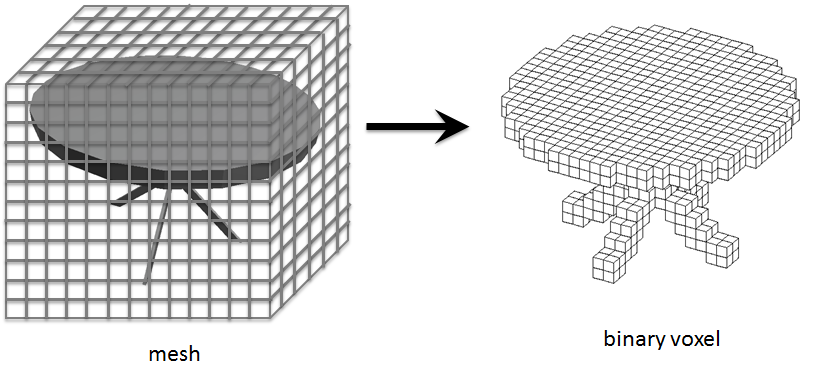
\includegraphics[width=\linewidth]{Voxel.png}
\end{center}
   \caption{Volumetric representation of a 3D object ~\cite{Authors14}}
\label{voxel}
\end{figure}

\begin{figure}[t] 
\begin{center}
	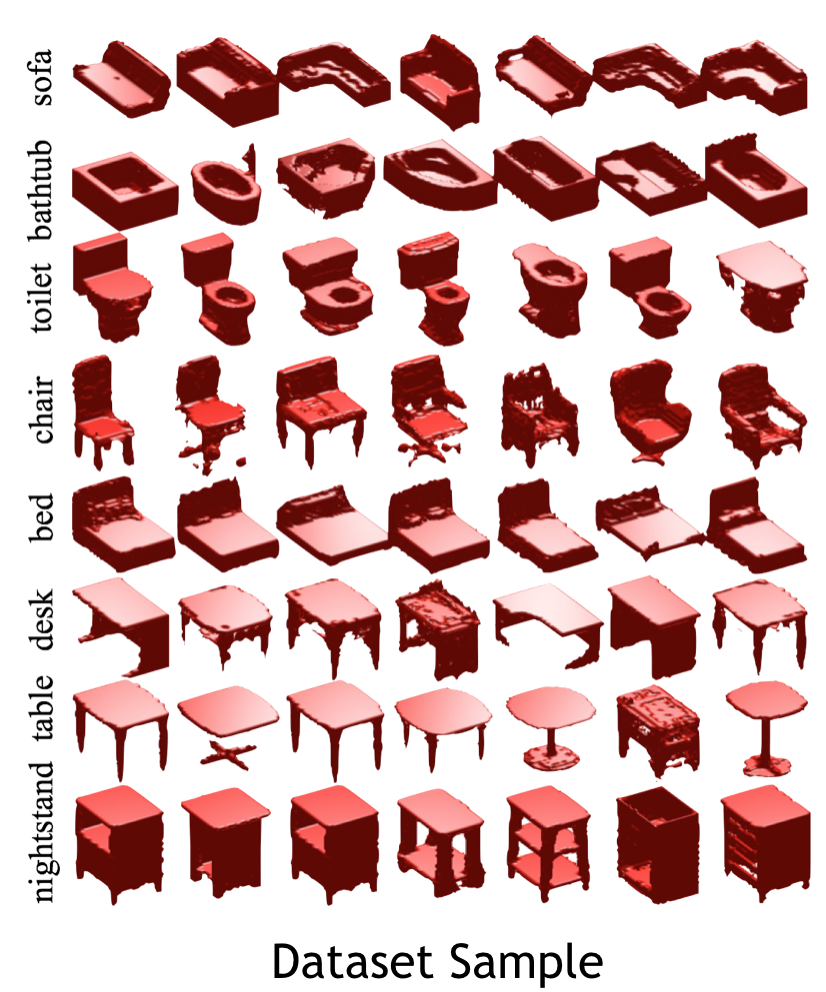
\includegraphics[width=\linewidth]{dataset_sample.png}
\end{center}
   \caption{Samples from the ModelNet40 dataset}
\label{dataset_sample}
\end{figure}


%-------------------------------------------------------------------------
\section{Results and Discussion}
\subsection{Model selection}
\subsubsection{Baseline architecture}
Our baseline (python) model has the following architecture:
convolution - ReLU - $2 \times 2$ max pool - affine - relu - affine - softmax. The hyper-parameters are: Filter size: $3 \times 3$, Number of Filters: 32, Learning Rate: $10^{-4}$, Regularization Strength: $10^{-5}$, Size of the hidden layer: 500. Update rule: Adam, Batch size: 50, Number of epochs: 1. The results are:\\
Training accuracy: 0.762\\
Validation accuracy: 0.772\\
Test accuracy: 0.725\\    
We note here that the test accuracy is considerably smaller then the training accuracy which suggests that our model is not generalizing well. This motivated us to include dropout layers in later architectures. The accuracy for 3DLayer V1 is slightly higher than for 3DLayer V2. We can say that the model for 3DLayer V1 with its lesser number of filters, is not over-fitting the training data compared to 3DLayer V2. This further strengthens our view that dropout is essential. 
\subsubsection{Novel architectures}

\begin{figure*}
\begin{center}
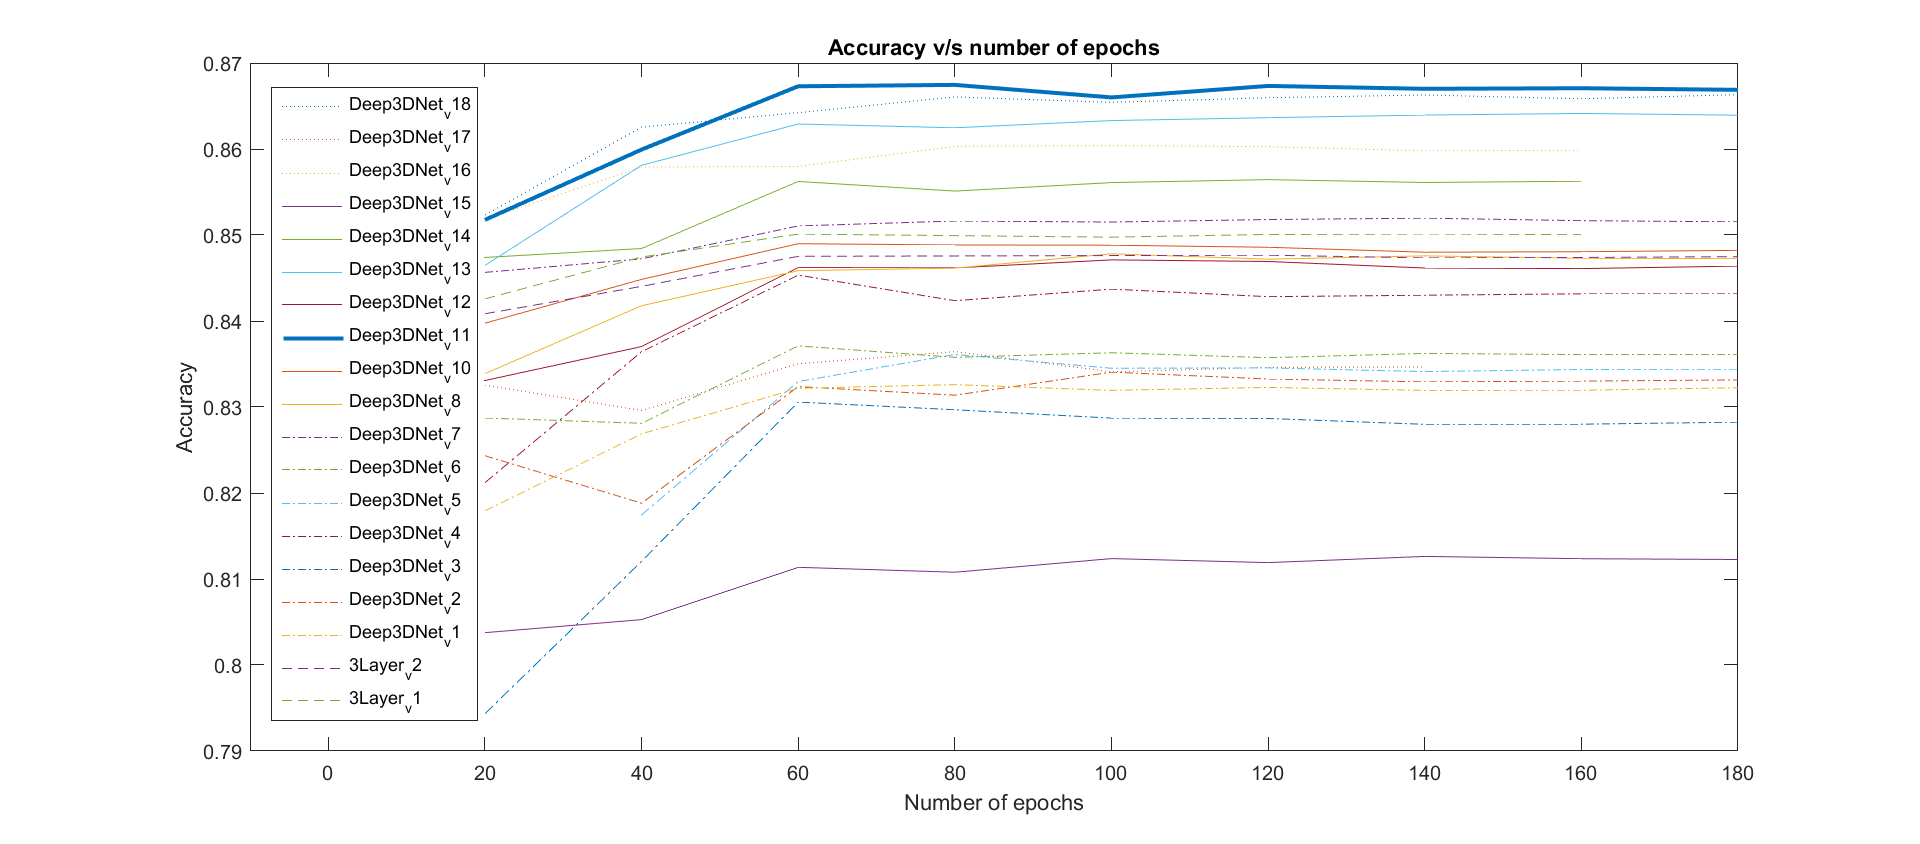
\includegraphics[width=\linewidth]{Model_Selection_Accuracy.png}
\end{center}
   \caption{Model Selection - Validation Accuracy v/s Epochs}
\label{model_accuracy}
\end{figure*}

\begin{figure*}
\begin{center}
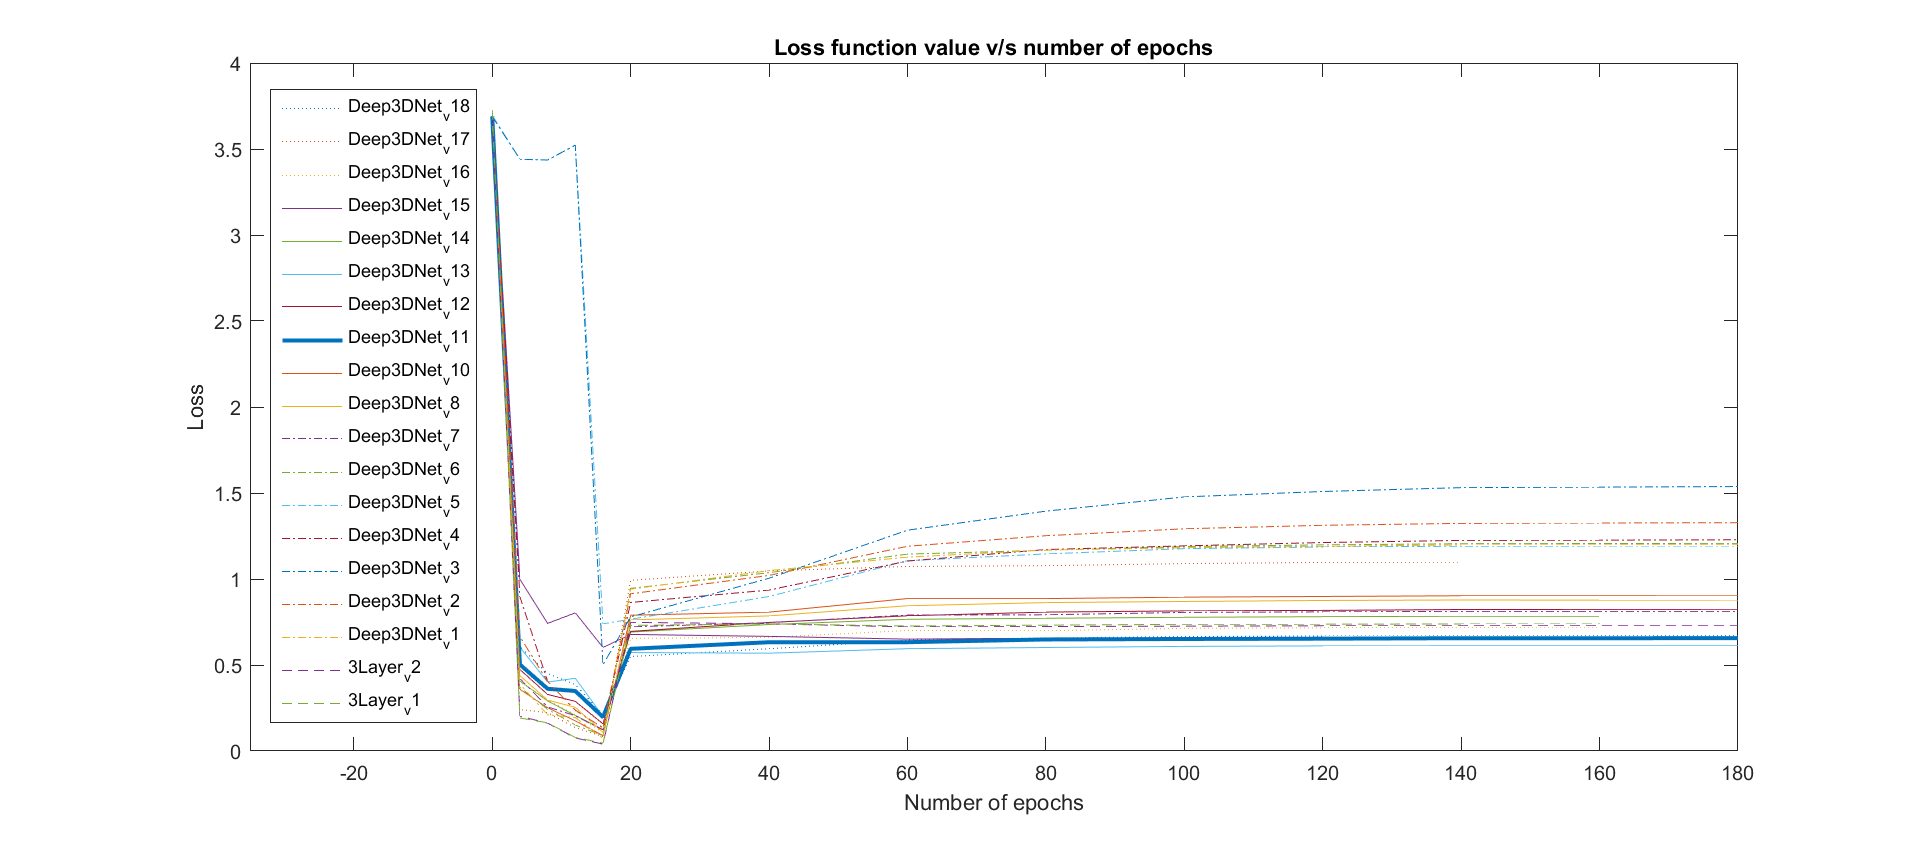
\includegraphics[width=\linewidth]{Model_Selection_Loss.png}
\end{center}
   \caption{Model Selection - Loss function v/s Epochs}
\label{model_loss}
\end{figure*}

\begin{figure}[t] 
\begin{center}
	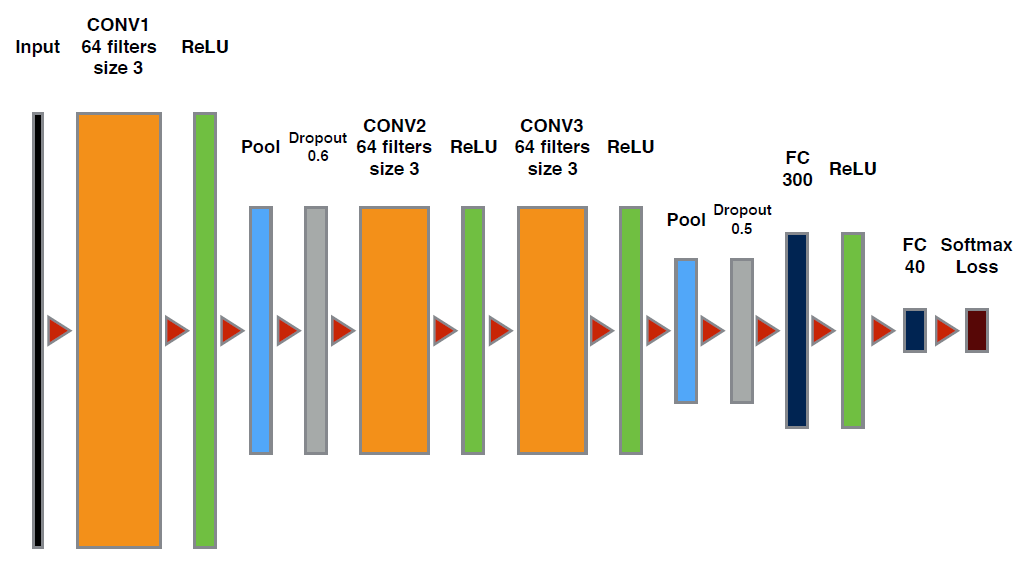
\includegraphics[width=\linewidth]{Best_model_arch.png}
\end{center}
   \caption{Best CNN model architecture and parameters}
\label{best_model}
\end{figure}

One of the general trends seen in all the models is that the validation accuracy curve plateaus after about 60 epochs. Similarly, the loss function plateaus after about 30 epochs. Also, the loss curves seem to go through a minimum before rising and flattening. It is interesting to note that the validation accuracy is not maximum for any model at the number of epochs for which the corresponding loss is minimum. Refer to Fig. \ref{model_accuracy} and Fig. \ref{model_loss} to note the following:\\ 
Observe that Deep3DNet V4 has significantly higher performance than V1,V2,V3,V5 and V6. We note that V1,V2,V3 and V6 are shallower networks compared to V4 and V5. Hence their generalizing power is lesser and they seem to be performing significantly below V4. Also V4 is the only model among V1,V2,V3,V6 which has a $1 \times 1$ convolutional layer. Comparing V4 and V5, V5 has two $1 \times 1$ convolutional layer layers instead of one in V4 and two $1 \times 1$ convolutional layer layers might be reducing the parameters significantly, thus degrading the performance of V5.\\
Observe that V7 beats all of the above models. This dramatic jump in performance is due to the introduction of the dropout layer. Dropout layers reduce over-fitting of the training data and improve validation performance.\\
Observe that V11, which is our winner, beats every model for epochs greater than 60. We note that V11 does not contain any $1 \times 1$ convolutional layer, and also does not contain any batch norm layers that were present in every model from V1 to V10. But V11 does contain two dropout layers. This may have led to its improved performance. V12 to V16 have the same architecture as V11, but different parameters. However, those parameters do not seem to be working as well as all of them report a lower validation accuracy. Note that V11 also has one of the least loss values for any epoch. Figure \ref{best_model} depicts the architecture and parameters of V11.\\ 
Observe that V17 has a significantly lower accuracy than V11. The only difference between them is that pooling layers have been removed from V17. This has increased the number of parameters by a huge amount and the performance has degraded. 

\subsection{Hyper-parameter tuning on best model}

\begin{table}
\begin{center}
\label{CNN_tuning}
\begin{tabular}{|c|c|c|c|}
\hline
Learning Rate & Weight Decay & Validation & Loss\\
\hline\hline
0.001 & 0.0005 & 0.84096 & 0.57086\\
0.001 & 0.005 & 0.84292 & 0.563102\\
0.001 & 0.05 & 0.744187 & 0.948633\\
0.001 & 0.5 & 0.048 & 3.67437\\
0.01 & 0.0005 & 0.861534 & 0.633144\\
0.01 & 0.005 & 0.867454 & 0.648504\\
0.01 & 0.05 & 0.734907 & 0.964328\\
0.01 & 0.5 & 0.048 & 3.67446\\
0.05 & 0.0002 & 0.865373 & 0.639149\\
0.05 & 0.0004 & 0.869533 & 0.582195\\
0.1 & 0.0005 & 0.868334 & 0.522467\\
0.1 & 0.005 & 0.842 & 0.507217\\
0.1 & 0.05 & 0.668293 & 1.17616\\
0.1 & 0.5 & 0.048 & 3.67468\\
0.15 & 0.00075 & 0.865547 & 0.496729\\
\textbf{0.15} & \textbf{0.001} & \textbf{0.873267} & \textbf{0.474882}\\
0.2 & 0.0002 & 0.783027 & 0.756309\\
0.2 & 0.0004 & 0.805147 & 0.65384\\
0.3 & 0.0002 & 0.0064 & 87.3364\\
0.3 & 0.0004 & 0.048 & 3.60804\\
0.4 & 0.0002 & 0.048 & 3.60809\\
0.4 & 0.0004 & 0.557373 & 1.47961\\
\hline
\end{tabular}
\end{center}
\caption{Hyper-parameter tuning for best CNN model}
\end{table}

As stated in Sec. \ref{sec:methods_section}, we have used SGD with momentum as our solver with a fixed momentum value of 0.9 as suggested by documentation of ~\cite{jia2014caffe}. We performed tuning over the learning rate and the weight decay (regularization) by maximizing the validation accuracy. First we did a course grid search for learning rate going from 0.001 to 0.1 and weight decay from 0.0005 to 0.5. Then, we did a finer search around our maxima. For each run, we trained the model for 50 epochs. The results can be seen in Table 1.  

\subsection{Training models for augmented datasets}

We chose the best hyper-parameters found in the above step, and trained the two augmented training sets. We did this for two reasons. One is that the data of the augmented training set comes from a similar distribution as the original training set (albeit with added noise). Secondly, performing hyper-parameter tuning is a highly compute and time expensive step and we were limited on both fronts. 

\subsection{Testing using best model for each training set}

\begin{table}
\begin{center}
\label{drop15_test_accuracy}
\begin{tabular}{|c|c|c|}
\hline
Iters & Accuracy & Loss     \\
\hline\hline
15000 & 0.84084  & 0.548466 \\
30000 & 0.857947 & 0.524602 \\
45000 & 0.863734 & 0.557168 \\
\textbf{60000} & \textbf{0.866467} & \textbf{0.545833} \\
\hline
\end{tabular}
\end{center}
\caption{Drop15 test accuracy}
\end{table}

\begin{table}
\begin{center}
\label{drop35_test_accuracy}
\begin{tabular}{|c|c|c|}
\hline
Iters & Accuracy & Loss     \\
\hline\hline
15000 & 0.827613 & 0.588618 \\
30000 & 0.850413 & 0.599797 \\
45000 & 0.8594   & 0.615183 \\
\textbf{60000} & \textbf{0.866587} & \textbf{0.573946} \\
\hline
\end{tabular}
\end{center}
\caption{Drop35 test accuracy}
\end{table}

For the original training set, our \textbf{best CNN reports a test accuracy of 0.841} with a loss of 0.5956 on the test set.\\
For Drop 15, which is the augmented training set with 15\% input dropout appended to the training set, we can see the test accuracy in Table 2. Note that this accuracy is higher than the accuracy for the best CNN on the original training set. This shows that augmenting the training data has enabled us to make the model more robust to noise and hence get more predictions right than before.\\
For Drop 35, which is the augmented training set with 35\% input dropout appended to the training set, we can see the test accuracy in Table 3. Note that this accuracy is higher than the accuracy for the best CNN on the original training set. This shows that augmenting the training data has enabled us to make the model more robust to noise and hence get more predictions right than before.\\
In both cases, we have expressed the performance as a function of training iterations and not epochs, because one epoch for the augmented training set is two epochs of the original training set and hence to avoid confusion, we have specified iteration count (at same batch size).

\subsection{Visualization of hidden layer features}

\begin{figure*}
\begin{center}
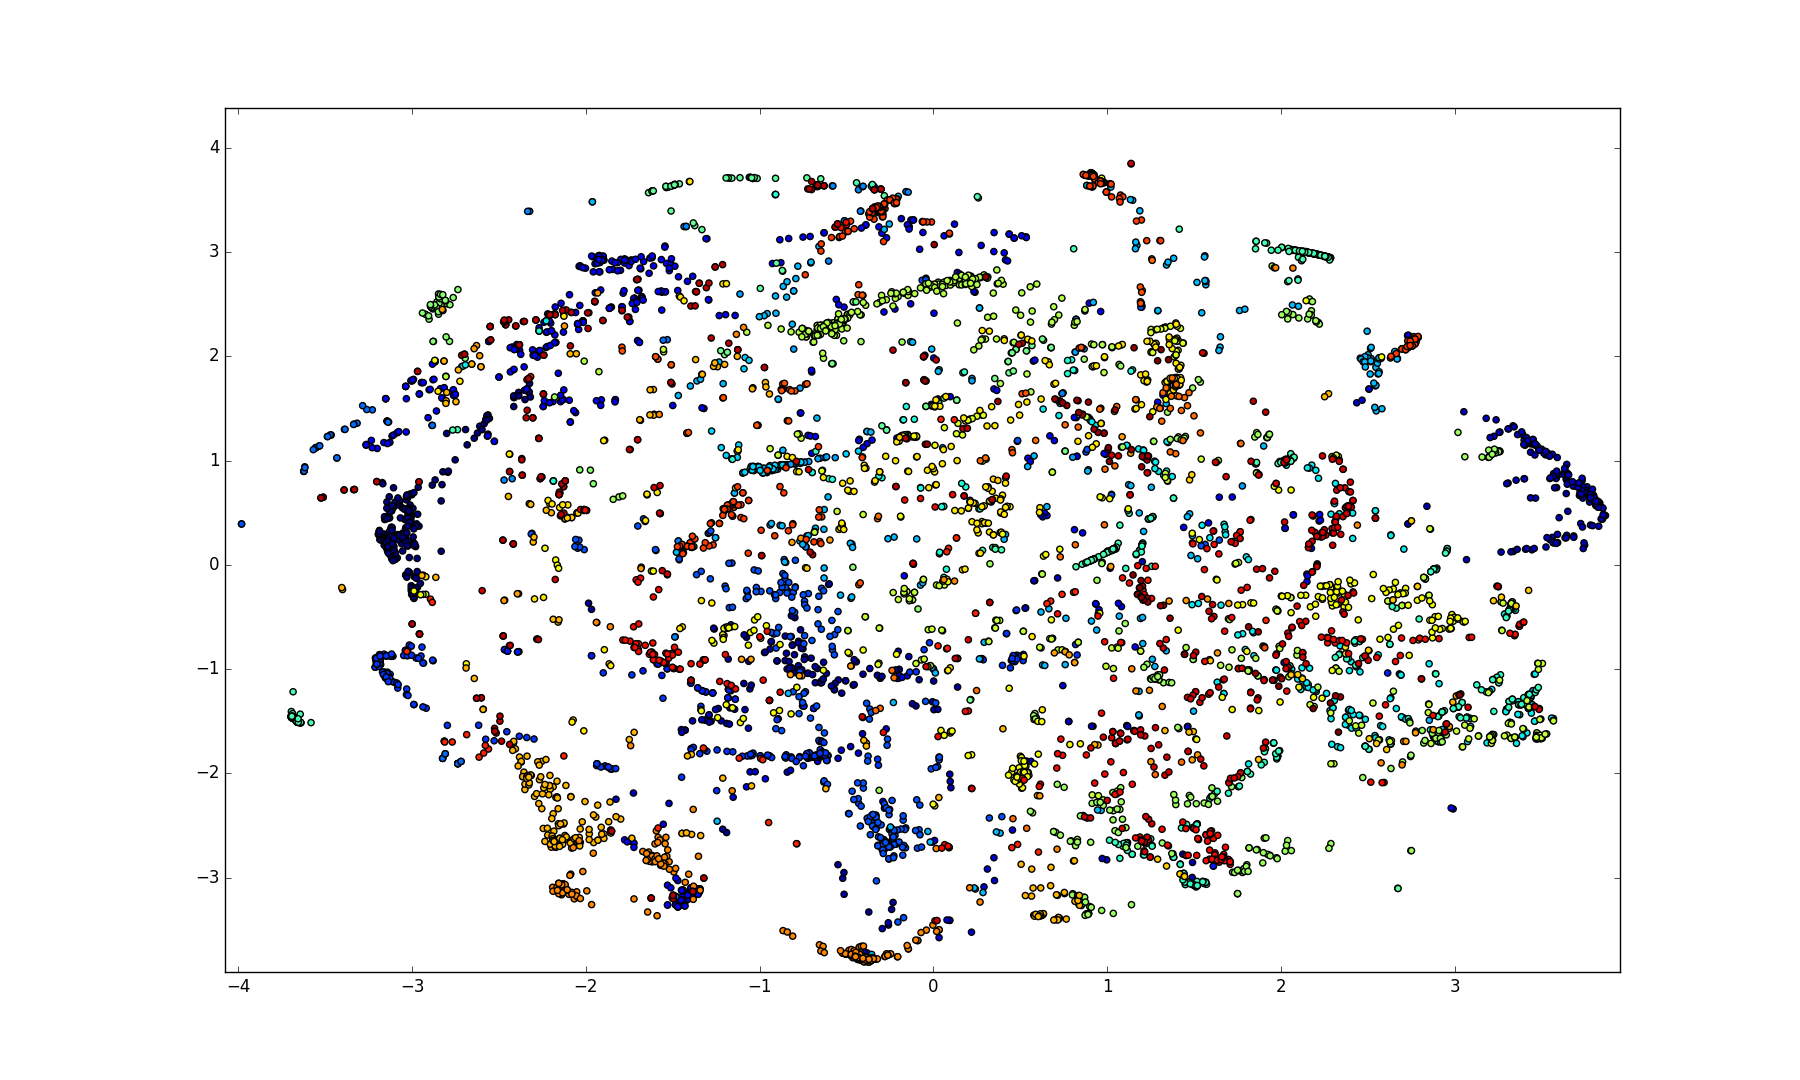
\includegraphics[width=\linewidth]{zoom_out.png}
\end{center}
   \caption{Visualization of hidden layer features using t-SNE}
\label{Visualization}
\end{figure*}

\begin{figure*}
\begin{center}
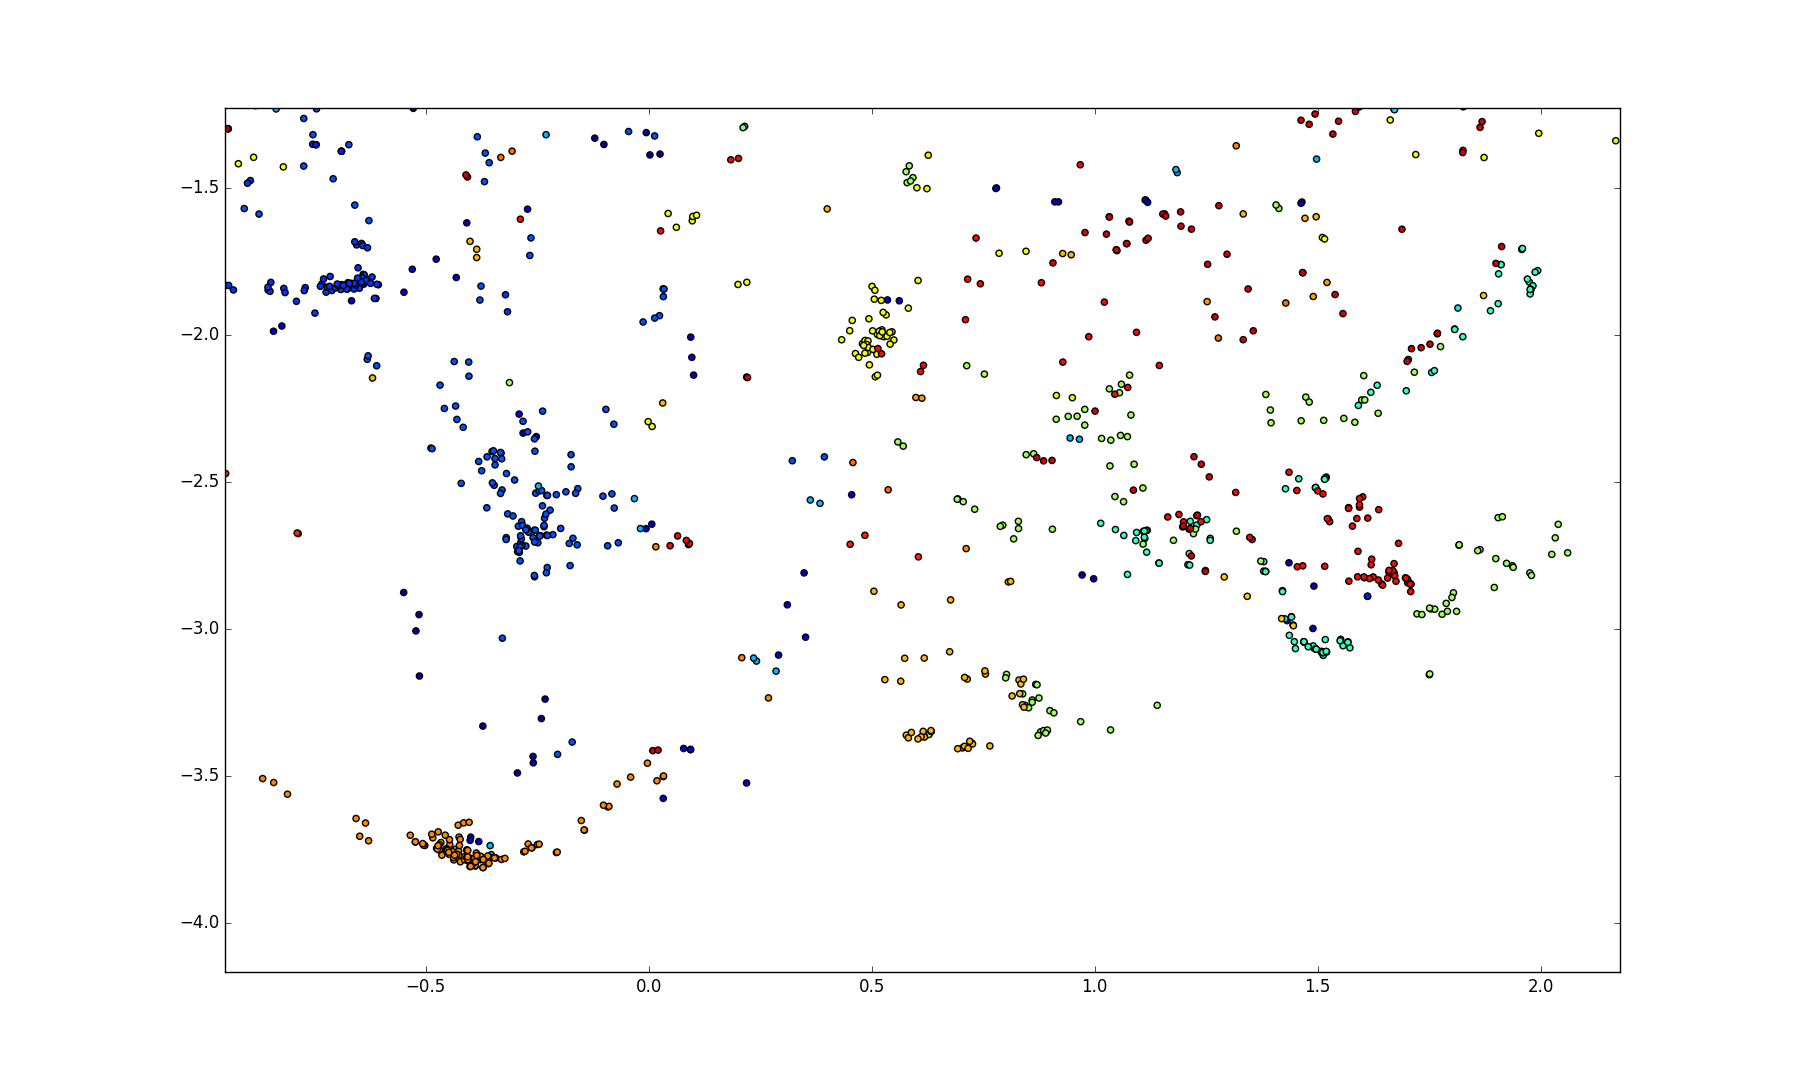
\includegraphics[width=\linewidth]{zoom2.png}
\end{center}
   \caption{Visualization of hidden layer features using t-SNE (Zoom in version)}
\label{Visualization2}
\end{figure*}


We have extracted 300 dimensional features from the hidden layer just prior to the last fully connected layer for about 14000 test examples and used t-SNE \cite{van2008visualizing} to create a 2D visualization as seen in Fig. \ref{Visualization} and Fig. \ref{Visualization2}. We can clearly see the yellow features clustered around (-2,-2), the aqua-marine features around (2,3) and the orange features around (-0.5, -4). This reassures us that the 300 dimensional hidden features of these classes were clustered together in the 300 dimensional space, hence allowing the linear classifier corresponding to the last fully connected layer in our CNN to predict the class labels. 

\subsection{SVM on hidden layer features}

\begin{table}
\begin{center}
\label{SVM_tuning}
\begin{tabular}{|c|c|c|}
\hline
$\gamma$             & C          & Validation Accuracy \\
\hline\hline
0.00001           & 0.1        & 0.8001              \\
0.000001          & 10         & 0.209288            \\
0.000001          & 0.1        & 0.853898            \\
0.0001            & 10         & 0.852813            \\
0.0001            & 10         & 0.862745            \\
0.00001           & 0.1        & 0.86666             \\
0.00001           & 1          & 0.7370169492        \\
0.000005          & 5          & 0.86586             \\
0.000005          & 50         & 0.86566             \\
\textbf{0.000015} & \textbf{5} & \textbf{0.8677966}  \\
0.000015          & 50         & 0.863796            \\
0.000005          & 25         & 0.866678            \\
0.000015          & 25         & 0.86525            \\
\hline
\end{tabular}
\end{center}
\caption{Hyper-parameter tuning for SVM}
\end{table}


\begin{figure}[t]
\begin{center}
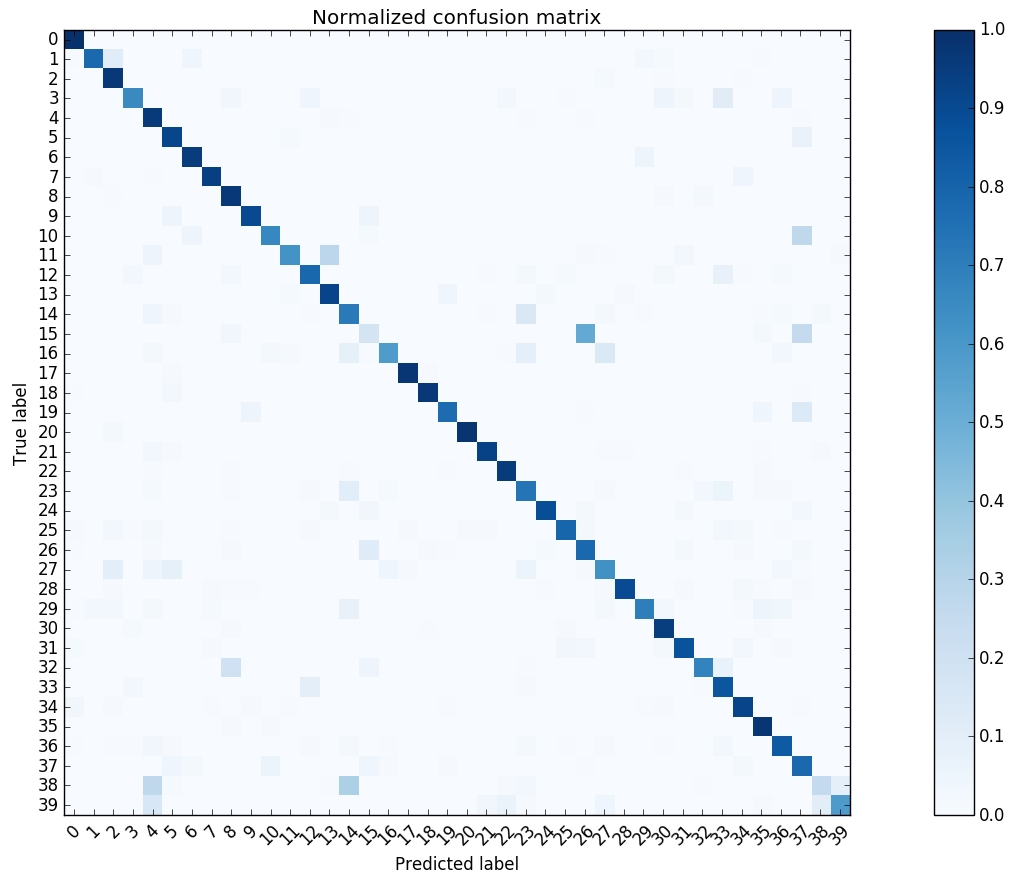
\includegraphics[width=\linewidth]{confusion_matrix.png}
\end{center}
   \caption{Confusion matrix for SVM}
\label{confusion_matrix}
\end{figure}

We employ the concept of 'transfer learning' to make use of our trained CNN as a feature descriptor and use the 300 dimensional hidden features as the input to our SVM. We select the RBF kernel and perform a course parameter grid search. We then select the best parameter combination and perform a finer grid search around it. The results can be seen in Table 4. In each case, we try to maximize the Top1 validation accuracy. The SVM that gave the best validation accuracy reports a test accuracy of 0.8513, which is higher than the test accuracy reported by our best CNN. Confusion matrix for this prediction can be seen in Fig. \ref{confusion_matrix}.



%-------------------------------------------------------------------------
\section{Conclusions and Future Work}
As a part of this project, we have trained 20 custom built CNNs and hyper-parameter tuning was carried out on the best model. This model was then trained on augmented data to make it more robust to noise. We have described and analyzed the performance of a few architectures we have trained. Our model Deep3DNet V11 gave the best test accuracy and we attribute this to it having dropout and pool layers. Also, V11 is significantly deeper than most of the other models. We also noted that training on the augmented dataset gave us higher test accuracy for both the augmented datasets. This is because our model becomes more robust to noisy input. We then trained an SVM on features extracted from one of the hidden layers of our best CNN and have reported a slightly higher test accuracy than our best CNN.\\
We have used $30 \times 30 \times 30$ binary voxel as our input. It is to be seen whether using a higher voxel resolution has any impact on classification accuracy. Using 3D convolutions instead of 2D convolutions might help boost accuracy. Inception modules can be added in the network (similar to ones used in GoogLeNet). Weight sharing can be implemented instead of dropout to make the network more robust.\\
The final aim of this project is to be build a real-time 3D object classification system. This is possible by integrating a NVIDIA-TX1 with a depth sensing camera like Intel RealSense and then loading our trained model on the TX1 to make real-time predictions. 
%------------------------------------------------------------------------


{\small
\bibliographystyle{ieee}
\bibliography{egbib}
}

\end{document}
